% ==============================================================================
% SECTION 1: INTRODUCTION AND CONTEXT
% ==============================================================================
\section{Introduction}

\begin{frame}{Project Objectives}
    \begin{columns}[c]
        % --- Left Column: Text Area ---
        \begin{column}{0.52\textwidth}
            \textbf{Available Resources:}
            \begin{itemize}
                \item Dataset of vertical acceleration.
                \item MATLAB/Simulink drone simulator.
            \end{itemize}

            \vspace{0.4em}
            \textbf{Objectives:}
            \begin{itemize}
                \item Validate the dataset.
                \item Identify the model.
                \item Develop a control law.
            \end{itemize}

        \end{column}

        % --- Right Column: 3 figures step_1, step_2, step_3 ---
        \begin{column}{0.45\textwidth}
            \centering
            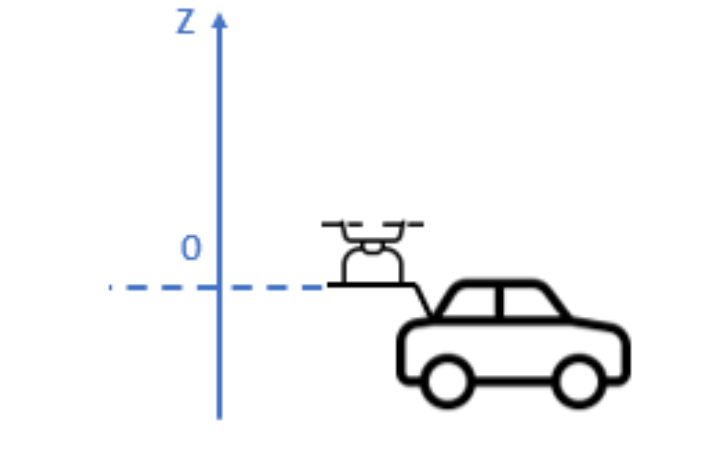
\includegraphics[width=\linewidth, height=2.1cm, keepaspectratio]{step_1.png}
            \vspace{0.3em}

            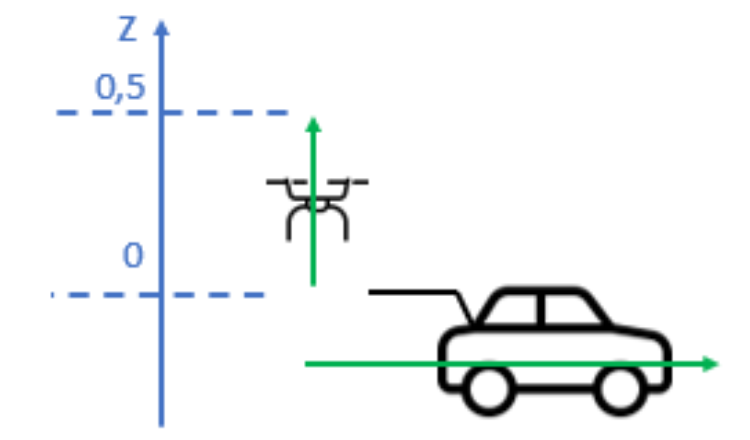
\includegraphics[width=\linewidth, height=2.1cm, keepaspectratio]{step_2.png}
            \vspace{0.3em}

            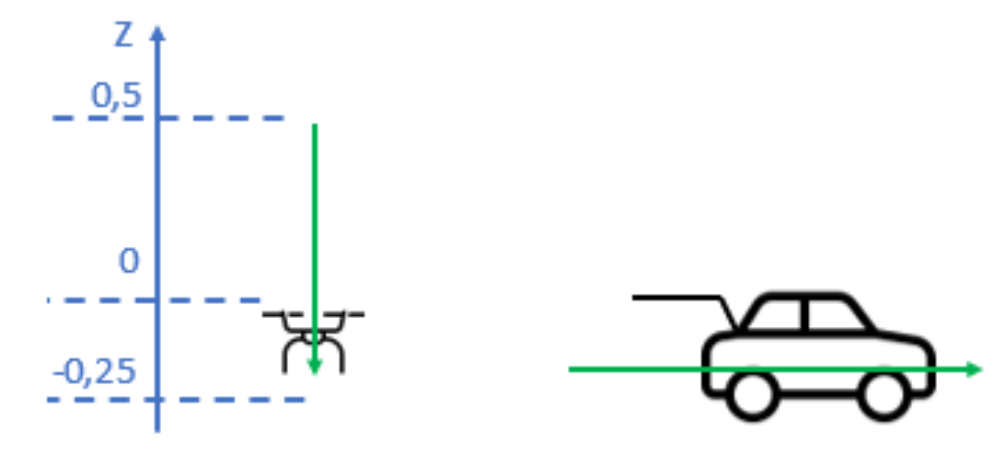
\includegraphics[width=\linewidth, height=2.1cm, keepaspectratio]{step_3.png}
        \end{column}
    \end{columns}
\end{frame}
